% =====================================================================
%  Paper 2: one fixed text prior for every camera, developed under
%  committed rules and tested once on an unseen benchmark.
%  Elsevier CAS single-column format (cas-sc). Extends Paper 1
%  (sarangi2026concept); shares references.bib and figures/ with it.
% =====================================================================

\documentclass[a4paper,fleqn]{cas-sc}

\usepackage[numbers,sort&compress]{natbib}
% Graphics are searched for beside this file and in figures/.
\graphicspath{{./}{figures/}}

\usepackage{amsmath,amssymb}
\usepackage{booktabs}
\usepackage{tabularx}
% rotating: the architecture figure sits on its own landscape page, where the
% text height is the available width, so it prints at full size and stays legible
\usepackage{rotating}
\usepackage{multirow}
\usepackage{algorithm}
\usepackage{algpseudocode}

\makeatletter
\@ifundefined{printorcid}{}{\renewcommand{\printorcid}{}}
\makeatother

% float placement: many tables and figures; keep each near its first mention
\renewcommand{\topfraction}{0.9}
\renewcommand{\bottomfraction}{0.8}
\renewcommand{\textfraction}{0.07}
\renewcommand{\floatpagefraction}{0.7}
\setcounter{topnumber}{3}
\setcounter{bottomnumber}{2}
\setcounter{totalnumber}{5}

\newcolumntype{Z}{>{\raggedright\arraybackslash}X}
\newcolumntype{W}[1]{>{\raggedright\arraybackslash}p{#1}}
\newcommand{\ci}[2]{\,[{#1},\,{#2}]}

% =====================================================================
\begin{document}
\let\WriteBookmarks\relax
\def\floatpagepagefraction{1}
\def\textpagefraction{.001}

\shorttitle{A frozen, camera-agnostic text prior for training-free video anomaly detection}
\shortauthors{P. K. Sarangi et~al.}

\title[mode = title]{Calm Words and Concrete Actions: A Frozen, Camera-Agnostic Text
Prior for Training-Free Video Anomaly Detection, Verified by a Sealed Test}

\author[1]{Prakash Kumar Sarangi}
% \cormark[1]
% \ead{prakash_m251250cs@nitc.ac.in}
\credit{Conceptualization, Methodology, Software, Investigation, Formal analysis,
Writing -- original draft}

\affiliation[1]{organization={National Institute of Technology Calicut},
    addressline={Department of Computer Science and Engineering},
    city={Kozhikode},
    postcode={673601},
    state={Kerala},
    country={India}}

\author[1]{Pranesh Das}
\credit{Supervision, Conceptualization, Writing -- review and editing}

\author[1]{Raju Hazari}
\credit{Supervision, Writing -- review and editing}

\begin{abstract}
Training-free video anomaly detectors compare frames with text, and the text is
usually tailored: to each camera, to each benchmark, or to each anomaly class. Our
earlier study found that a description written for each camera mostly calibrates
cameras against one another and fails when the frames it is written from already
show the event. We therefore ask whether one fixed piece of text, the same for every
camera and every dataset, can carry a frozen detector instead. The model pairs a
frozen PE-Core encoder with eight calm, low-motion normal phrases and a bank of 48
concrete actions in twelve types; it uses no captioning model, no per-camera input
and no gradient update. It was developed one change at a time under rules committed
before each step, on ShanghaiTech, UCF-Crime, XD-Violence and NWPU Campus, where it
reaches $0.783$, $0.856$, $0.722$ (average precision) and $0.639$; on XD-Violence it
exceeds the description-based system by $+0.305$ $[+0.255, +0.359]$. The calm phrases
help on PE-Core but do nothing on CLIP ViT-L/14, and on two benchmarks, unlike scene
descriptions, they mainly re-rank frames within each video. Before any data from a fifth benchmark was
obtained, the model, the evaluation and the permitted wording of every outcome were
frozen. On the official UBnormal test split, scored once, the model reaches a micro
AUROC of $0.747$ $[0.704, 0.789]$, $+0.096$ $[+0.051, +0.142]$ above plain PE-Core, and
all three pre-registered predictions hold.
\end{abstract}

\begin{highlights}
\item One fixed set of 59 phrases replaces text written for each camera
\item Calm normal phrases help on PE-Core but do nothing on CLIP ViT-L/14
\item On two benchmarks the calm phrases re-rank frames, unlike scene descriptions
\item Model, metrics and wording were frozen before any test data was obtained
\item Sealed UBnormal test: 0.747 AUROC, all three predictions hold
\end{highlights}

\begin{keywords}
video anomaly detection \sep training-free detection \sep vision-language models
\sep prompt design \sep pre-registration \sep sealed evaluation
\end{keywords}

\maketitle

% =====================================================================
\section{Introduction}
\label{sec:intro}
% =====================================================================

A surveillance network may run hundreds of cameras, each watching a different place.
A detector that must be retrained, re-tuned or re-described for each of them does not
scale, which is why training-free video anomaly detection (VAD) has drawn attention:
a frozen vision-language model compares each frame with a few sentences, and nothing
is learned on the target site
\citep{zanella2024lavad, anyanomaly2025, yin2026nova, lee2025flashback, zou2026askhint}.
The sentences then do the work that training used to do, and the question becomes
who writes them and for what.

Our first study \citep{sarangi2026concept} examined one answer: describe each camera's
scene in a sentence, written by an operator or by a captioning model from the
camera's first frames, and add it to the normal side of the prompts. Measured with a
falsifiable protocol, the description was load-bearing but fragile. Most of its
benefit was calibration, which moves each camera's scores as a block, rather than
better ranking of frames within a video. And on XD-Violence it failed outright,
lowering average precision from $0.624$ to $0.417$, because in a quarter of the
violent videos the frames it was written from already showed the violence.

This paper takes the opposite approach. Instead of writing text for each camera, we
fix one text prior for all of them: a description of what calm, ordinary footage
looks like, and a list of concrete things that go wrong. Nothing about it depends on
a camera's opening frames, so the failure mode above cannot arise, and a new camera
needs no input at all. The price is that the text cannot adapt to a site, and the
open question is whether one fixed list can serve campus walkways, shop interiors,
films and rendered scenes alike.

Answering that question honestly is harder than it looks, because a fixed list is
easy to over-fit to the benchmarks used to write it. We therefore separate
development from testing as strictly as we could. Every change was made one at a
time, with its rules and predictions committed to the repository before it was
scored. When development ended, the model's files, the evaluation and the exact
wording permitted for each possible outcome were frozen. Only then was a fifth
benchmark, UBnormal \citep{acsintoae2022ubnormal}, downloaded and scored, once.

\paragraph{Contributions.}
\begin{enumerate}[(1)]
  \item \textbf{A camera-agnostic text prior.} Eight calm, low-motion normal phrases,
        following the normality rules of NOVA \citep{yin2026nova} but with no
        reference drawn from the target video, and a frozen bank of 48 concrete
        actions in twelve types, used unchanged on every camera and every dataset with
        a frozen PE-Core encoder \citep{bolya2025pe} (Section~\ref{sec:method}).
  \item \textbf{What the text does, measured.} The calm phrases are
        encoder-dependent, helping PE-Core on three of four benchmarks and CLIP
        ViT-L/14 on none, and on ShanghaiTech and NWPU Campus they mainly re-rank
        frames within a video, which scene descriptions did not
        (Section~\ref{sec:dev}).
  \item \textbf{A sealed test.} A complete evidence chain, from committed rules for
        each development step to a single scored run on a benchmark obtained after
        freezing, with every number and every claim fixed in advance
        (Sections~\ref{sec:protocol} and~\ref{sec:sealed}).
  \item \textbf{A record of what failed, and an ablation of what remains.} Scoring by
        anomaly type, scene-chosen phrases, per-side templates, a camera memory and
        encoder averaging all failed the development rule, and are reported with their
        numbers (Section~\ref{sec:dev-failed}); an ablation of the frozen model shows
        that both ingredients are needed on unseen data and that the bank works by
        breadth (Section~\ref{sec:ablation}).
\end{enumerate}

% =====================================================================
\section{Related Work}
\label{sec:related}
% =====================================================================

\paragraph{Where the text comes from in training-free VAD.}
Training-free detectors differ less in their encoders than in their text. LAVAD
captions every frame and asks a large language model to score the captions
\citep{zanella2024lavad}. AnyAnomaly lets the user name the anomaly of interest and
queries a large vision-language model several times per segment
\citep{anyanomaly2025}. NOVA strengthens the normal side: it excludes anomaly-adjacent verbs from normal
prompts, biases normal descriptions toward static, low-motion scenes, and adds a
visual normal anchor built from the initial frames of each test video
\citep{yin2026nova}. ASK-Hint organises fine-grained, action-centric guiding questions into groups of
anomaly categories and poses them to a frozen vision-language model
\citep{zou2026askhint}. Flashback has a language model build a memory of normal and
anomalous captions offline and matches video segments against it, with no language
model at inference \citep{lee2025flashback}, and \citet{song2026vlmanswer} show that a model's yes/no
answer is a poor ranking score unless its probabilities are used. Our first study
supplied a description of each camera's scene \citep{sarangi2026concept}.
Table~\ref{tbl:position} places these methods by what their text requires.

\begin{table}[width=\linewidth,cols=4,pos=htbp]
\caption{Training-free detectors by the text they use. ``From the target video'': the
text or the normal reference is derived from the video being scored. ``Large model at
test'': a language or vision-language model is queried during detection. Entries
follow each paper's own description of its method.}\label{tbl:position}
\small
\begin{tabularx}{\linewidth}{@{}l Z c c@{}}
\toprule
\textbf{Method} & \textbf{Text and normal reference} & \textbf{From the target video} & \textbf{Large model at test} \\
\midrule
LAVAD \citep{zanella2024lavad} & captions of the video's frames, scored by an LLM & yes & yes \\
AnyAnomaly \citep{anyanomaly2025} & anomaly named by the user & no & yes \\
NOVA \citep{yin2026nova} & low-motion normal prompts; visual anchor from each video's initial frames & yes & no \\
ASK-Hint \citep{zou2026askhint} & guiding questions grouped by anomaly category & no & yes \\
Flashback \citep{lee2025flashback} & memory of LLM-generated captions, built offline & no & no \\
Scene description \citep{sarangi2026concept} & a caption of each camera's first frames & yes & no \\
\textbf{This work} & \textbf{59 fixed phrases, the same for every camera} & \textbf{no} & \textbf{no} \\
\bottomrule
\end{tabularx}
\end{table}

Table~\ref{tbl:litsum} summarises the works this paper builds on: for each, its year
and venue, its central idea, and the limitation that matters for a text prior that must
be fixed in advance and serve every camera.

\begin{table}[width=\linewidth,cols=5,pos=htbp]
\caption{Works this paper builds on, read from the standpoint of a fixed,
camera-agnostic text prior. The last column is the property that work lacks for that
purpose, not a general criticism of it.}\label{tbl:litsum}
\footnotesize
\begin{tabularx}{\linewidth}{@{}W{2.3cm} l W{1.5cm} Z Z@{}}
\toprule
\textbf{Work} & \textbf{Year} & \textbf{Venue} & \textbf{Central idea} & \textbf{Missing for a fixed, camera-agnostic prior} \\
\midrule
CLIP \citep{radford2021clip} & 2021 & ICML & Contrastive image--text space; zero-shot labels from text & Text must still be chosen for the task \\
UBnormal \citep{acsintoae2022ubnormal} & 2022 & CVPR & Rendered benchmark whose test anomalies differ from its training ones & A benchmark, not a method; used here as the sealed test \\
WinCLIP \citep{jeong2023winclip} & 2023 & CVPR & Normal and abnormal prompt ensembles for zero-shot defects & Industrial images; no notion of scene or time \\
LAVAD \citep{zanella2024lavad} & 2024 & CVPR & Captions of every frame, scored by a language model & Text derived from each target video; heavy at test time \\
AnomalyRuler \citep{yang2024anomalyruler} & 2024 & arXiv & Rules of normality induced by GPT-4 from a few normal frames & Needs frames of the target scene \\
VERA \citep{ye2025vera} & 2025 & CVPR & Guiding questions learned on training videos & Text optimised on labelled data \\
Flashback \citep{lee2025flashback} & 2025 & arXiv & Retrieval from a memory of generated captions & A large memory and a video encoder \\
PE-Core \citep{bolya2025pe} & 2025 & NeurIPS & A stronger contrastive image--text encoder & An encoder, not a text prior \\
AnyAnomaly \citep{anyanomaly2025} & 2026 & WACV & The user names the anomaly to look for & The anomaly classes must be known in advance \\
ASK-Hint \citep{zou2026askhint} & 2026 & WACV & Action-centric questions to a large vision-language model & A large model queried at test time \\
NOVA \citep{yin2026nova} & 2026 & arXiv & Calm, low-motion normal prompts; visual anchor per video & Phrases written per anomaly class; anchor from each test video \\
Song and Lee \citep{song2026vlmanswer} & 2026 & arXiv & A model's yes/no answer compresses the ranking & Concerns the score, not the text \\
\bottomrule
\end{tabularx}
\end{table}

\paragraph{Normal-side modelling.} Describing normality rather than enumerating
anomalies has a long history in one-class VAD, where a model of normal footage is
learned from the target site \citep{liu2018shanghaitech, lv2021mpn, micorek2024mulde}.
In training-free work, NOVA is the direct precedent for our normal side: its
normality-aware prompts exclude anomaly-adjacent verbs and favour static, low-motion
scenes \citep{yin2026nova}. Our calm phrases follow those two rules; we wrote our own
phrases rather than using NOVA's generated ones, and we omit its visual anchor, which
is computed from each test video's initial frames. Our earlier normal-side experiment
had broken the first rule, by adding look-alike actions such as hugging beside
fighting, and the present design corrects it.

\paragraph{Encoders.} CLIP \citep{radford2021clip} and its open reproductions are the
default encoders for zero-shot anomaly scoring \citep{jeong2023winclip,
zhou2024anomalyclip}. The Perception Encoder (PE-Core) is a more recent contrastive
image--text model whose strongest features lie inside the network rather than at its
output \citep{bolya2025pe}; Flashback reports its best results with it
\citep{lee2025flashback}. We use PE-Core's output embedding, frozen.

\paragraph{Development reuse and sealed tests.} Every benchmark in a VAD study is
usually used both to choose a method and to report it, and the published comparison
tables of the methods above are built that way. The risk is familiar: a design chosen
among many variants on the same test videos will look better there than on new data.
A held-out benchmark, scored once under conditions fixed in advance, is the direct
remedy. We know of no training-free VAD study that reports one, and we do so here.

% =====================================================================
\section{From Scene Descriptions to a Fixed Text Prior}
\label{sec:lessons}
% =====================================================================

The first study left four lessons, each of which becomes a requirement here.

\begin{enumerate}[L1.]
  \item \emph{Text written from a camera's opening frames inherits whatever those
        frames show.} On XD-Violence, removing the description from only the 127
        videos whose opening frames contained violence recovered two thirds of the
        loss \citep{sarangi2026concept}.
  \item \emph{The point at which text enters matters more than its wording.} Adding
        the same text to both prompt ensembles drew their mean embeddings together
        and reversed the effect.
  \item \emph{A description mostly calibrates.} Between $82\%$ and $87\%$ of its
        gains were a shift in each video's score level.
  \item \emph{A wrong description is worse than none.} Giving each video another
        video's description cost more than supplying no text at all.
\end{enumerate}

From these follow four requirements for the text prior.

\begin{enumerate}[R1.]
  \item \textbf{No dependence on the target's footage} (L1, L4): the text is written
        once and is identical for every camera.
  \item \textbf{Separate sides} (L2): normal and abnormal phrases share no wording,
        so the two mean embeddings are not drawn together.
  \item \textbf{Ranking, not only calibration} (L3): the text should help order frames
        within a video, which a per-camera offset cannot do.
  \item \textbf{No model at test time}: detection costs one image-encoder pass per
        sampled frame, and the text is encoded once.
\end{enumerate}

\subsection{Problem setting}
\label{sec:setting}
A video is a sequence of frames $X=(x_1,\dots,x_T)$ with frame labels
$y_t\in\{0,1\}$, where $1$ marks an anomaly; labels are used only for evaluation. A
\emph{text prior} is a pair of phrase sets $\mathcal{T}=(P^{+},P^{-})$, normal and
abnormal. A training-free detector with frozen parameters $\theta$ maps a video and a
text prior to one score per frame,
\begin{equation}
\tilde{s}_{1:T} \;=\; f_\theta\big(X;\,\mathcal{T}\big), \qquad \theta\ \text{fixed}.
\label{eq:detector}
\end{equation}
The first study let the text depend on the camera, $\mathcal{T}=\mathcal{T}(c_k)$,
with $c_k$ a description written from camera $k$'s opening frames. Here the text prior is
\emph{camera-agnostic}: one $\mathcal{T}$ for every camera and every dataset, chosen
before any target video is seen (R1). Choosing it is itself a selection problem, so the
benchmarks are split by role. A development set $\mathcal{D}_{\mathrm{dev}}$ (four
benchmarks) is used to choose $\mathcal{T}$ under a rule $\mathcal{R}$ fixed in advance,
and a sealed test set $\mathcal{D}_{\mathrm{test}}$ (UBnormal) is used once, after the
choice is frozen:
\begin{equation}
\mathcal{T}^{\star} = \mathcal{R}\big(\{\mathcal{T}_1,\mathcal{T}_2,\dots\};\,
\mathcal{D}_{\mathrm{dev}}\big), \qquad
\text{reported:}\ \ M\big(f_\theta(\cdot\,;\mathcal{T}^{\star});\,\mathcal{D}_{\mathrm{test}}\big),
\label{eq:selection}
\end{equation}
where $M$ is the evaluation measure (Section~\ref{sec:metrics}). Figures on
$\mathcal{D}_{\mathrm{dev}}$ guided the choice and are exploratory; only the figure on
$\mathcal{D}_{\mathrm{test}}$ estimates how the frozen prior performs on new data.

% =====================================================================
\section{Method}
\label{sec:method}
% =====================================================================

\subsection{Overview}
Figure~\ref{fig:arch2} shows the detector. A frozen image encoder embeds each sampled
frame. Two fixed sets of phrases, normal and abnormal, are embedded once by the
matching text encoder and averaged into one prototype per side. Each frame's score is
how much closer it lies to the abnormal prototype than to the normal one, smoothed
over a short window. Every component is frozen, the 59 phrases are the same for every
camera, and nothing is computed from the target site before detection begins.

\begin{sidewaysfigure}
\centering
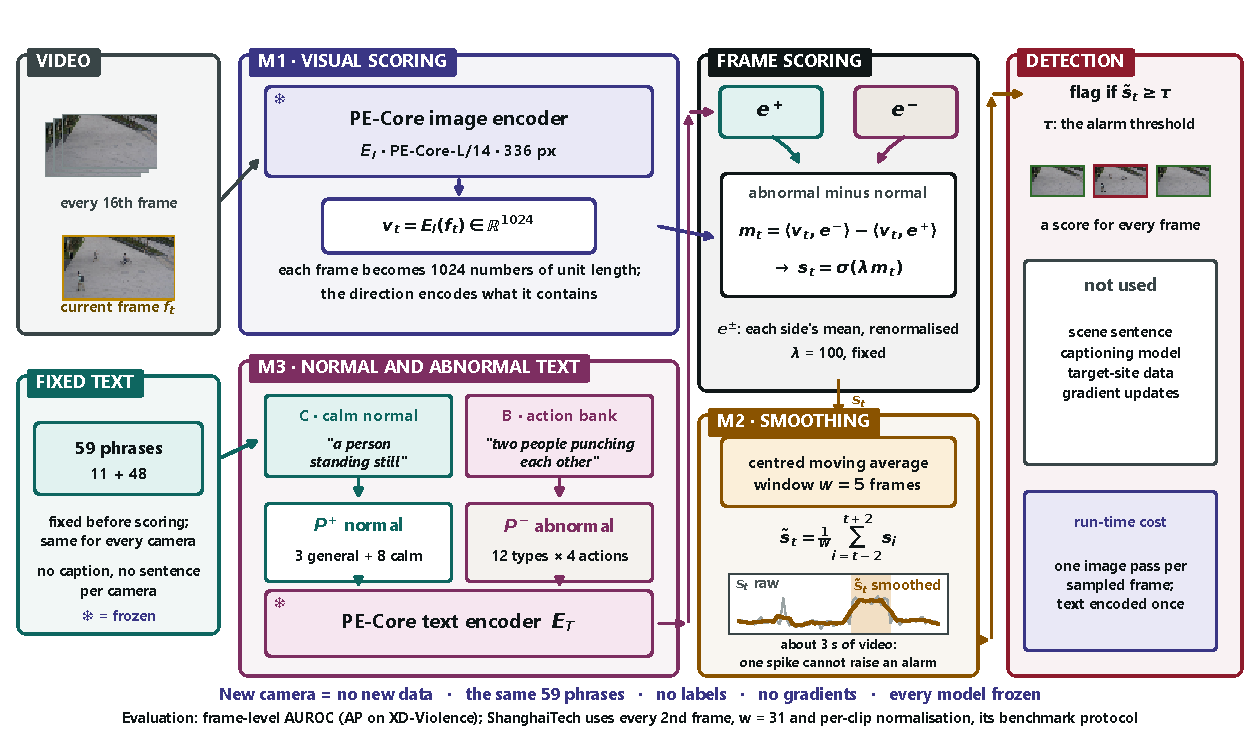
\includegraphics[width=0.97\textheight]{fig_architecture_final}
\caption{The detector. M1: a frozen PE-Core image encoder at $336\times336$ pixels.
M3: the normal ensemble (three general phrases and eight calm phrases, C) and the
abnormal ensemble (48 concrete actions in twelve types, B), embedded once by the
frozen text encoder. Frame scoring: the margin between the two prototypes, passed
through a sigmoid. M2: a centred moving average. The right-hand panel lists what the
model does not use.}\label{fig:arch2}
\end{sidewaysfigure}

\subsection{Encoder}
The image and text encoders are PE-Core-L/14 at $336\times336$ pixels
\citep{bolya2025pe}, used through \texttt{open\_clip} with all weights frozen.
Each sampled frame $f_t$ becomes a unit vector $v_t\in\mathbb{R}^{1024}$; each
phrase $p$ becomes a unit vector $u(p)$ in the same space. The encoder's learned logit
scale is $99.9$; we keep $\lambda=100$, as in the first study.

\subsection{Normal side: calm, low-motion phrases}
The normal ensemble $P^{+}$ holds the three general surveillance phrases of the first
study and eight calm phrases (Table~\ref{tbl:normal}): four quiet places and four
people doing nothing in particular. They follow the two rules of NOVA's normality-aware prompts \citep{yin2026nova}: no
normal phrase names or resembles an anomalous action, and normal phrases describe
static, low-motion scenes. The phrases are our own, written without any list of
anomaly classes. A second
wording with no phrase in common was written at the same time and is used only to
check that the effect does not hinge on particular words
(Section~\ref{sec:dev-effects}).

\begin{table}[width=\linewidth,cols=3,pos=htbp]
\caption{The normal ensemble $P^{+}$. The second wording was used only as a robustness
check and is not part of the model.}\label{tbl:normal}
\small
\begin{tabularx}{\linewidth}{@{}l Z Z@{}}
\toprule
\textbf{Group} & \textbf{Phrases in the model} & \textbf{Second wording (check only)} \\
\midrule
General (3) & a normal day with people behaving ordinarily; a calm and safe public area; nothing dangerous or abnormal is happening & --- \\
\addlinespace
Quiet places (4) & an empty walkway; an empty street; an empty room; a quiet open area with nobody around & a deserted pavement; an unoccupied hallway; a vacant plaza; a still courtyard with no one in it \\
\addlinespace
Calm people (4) & a person standing still; a person sitting quietly; two people talking calmly; a person walking slowly & someone waiting patiently; a person resting on a bench; a few people chatting quietly; someone strolling at an easy pace \\
\bottomrule
\end{tabularx}
\end{table}

\subsection{Abnormal side: a frozen bank of concrete actions}
The abnormal ensemble $P^{-}$ replaces abstract phrases such as ``an abnormal and
unsafe situation'' with 48 concrete actions, four for each of twelve types
(Table~\ref{tbl:bank}). Concrete actions follow the finding of ASK-Hint that frozen
models judge actions better than labels \citep{zou2026askhint}. The bank was written
once by a large language model, read, committed, and then frozen before it was first
scored; it was never edited after a score was seen. The same 48 phrases are used for
every benchmark, including ones whose anomalies are of quite different kinds.

\begin{table}[width=\linewidth,cols=2,pos=htbp]
\caption{The abnormal ensemble $P^{-}$: twelve types, four concrete actions each.
Fixed before first use and identical for every camera and every
benchmark.}\label{tbl:bank}
\footnotesize
\begin{tabularx}{\linewidth}{@{}W{2.9cm} Z@{}}
\toprule
\textbf{Type} & \textbf{Phrases} \\
\midrule
Fighting & two people punching each other; a person kicking someone on the ground; a group of people brawling; a person violently shoving another person \\
Weapon & a person pointing a gun at someone; a person firing a gun; a person threatening someone with a knife; a person stabbing someone \\
Theft & a person snatching a bag from someone; a robber holding up a cashier; a person stealing goods from a shop; a burglar climbing through a window \\
Vandalism & a person smashing a window; a person kicking a door open; a person damaging a parked car; a person spraying graffiti on a wall \\
Road accident & two cars crashing into each other; a car hitting a pedestrian; a motorcycle skidding across the road; a vehicle overturned on the road \\
Fire or explosion & flames and thick smoke rising from a building; a car on fire; an explosion with debris flying; a blast throwing people to the ground \\
Riot or arrest & a crowd of rioters throwing objects; a mob clashing with police; police wrestling a person to the ground; a person being handcuffed and arrested \\
Abuse & an adult hitting a child; a person dragging another person by force; a person being beaten while lying down; a person being grabbed and restrained \\
Falling & a person collapsing to the ground; a person lying motionless on the ground; a person falling from a height; a person tripping and falling hard \\
Vehicle among pedestrians & a cyclist riding through a crowd of pedestrians; a car driving on a pedestrian walkway; a motorbike riding on a footpath; a person on a skateboard weaving between pedestrians \\
Sudden running & a person sprinting through a crowd; a person chasing someone; people running away in panic; a person jumping over a barrier \\
Trespass & a person climbing over a fence; a person forcing entry into a restricted area; a person leaving a suspicious bag behind; a person hiding and watching people \\
\bottomrule
\end{tabularx}
\end{table}

\subsection{Scoring and smoothing}
Each side's phrase embeddings are averaged and renormalised,
\begin{equation}
e^{\pm} \;=\; \frac{\sum_{p\in P^{\pm}} u(p)}{\big\|\sum_{p\in P^{\pm}} u(p)\big\|},
\label{eq:proto}
\end{equation}
and each frame receives the margin and score
\begin{equation}
m_t \;=\; \langle v_t, e^{-}\rangle - \langle v_t, e^{+}\rangle, \qquad
s_t \;=\; \sigma(\lambda\, m_t),
\label{eq:margin}
\end{equation}
where $\sigma$ is the logistic function; this equals the two-way softmax over the two
scaled similarities. The scores are smoothed by a centred moving average of $w$
sampled frames, in which the first and last scores of a video are repeated to fill the
window at its ends,
\begin{equation}
\tilde{s}_t \;=\; \frac{1}{w}\sum_{j=-\lfloor w/2\rfloor}^{\lfloor w/2\rfloor}
s_{\min(T,\,\max(1,\,t+j))};
\label{eq:smooth2}
\end{equation}
for a video shorter than $w$ sampled frames, $w$ is set to its length.
Every sixteenth frame is scored and $w=5$ (about three seconds of video at 25--30
frames per second). ShanghaiTech keeps its benchmark protocol: every second frame,
$w=31$ and min--max normalisation of each clip before pooling. On every other
benchmark scores are pooled raw.

\subsection{Cost and what the model does not use}
Detection costs one image-encoder pass per sampled frame and two inner products; the
59 phrases are encoded once. The model uses no captioning or language model, no
description of the site, no frames or labels from the target benchmark, and no
gradient update. A new camera is connected and scored with no input beyond its video.

\subsection{Inputs and outputs}
\label{sec:io2}
Table~\ref{tbl:io2} lists what the detector consumes and returns. Two things are
absent from the input column that were present in the first study: a description of the
scene, and any frame of the target camera used before detection.

\begin{table}[width=\linewidth,cols=3,pos=htbp]
\caption{What the detector consumes and returns. $D=1024$ for PE-Core-L/14.}\label{tbl:io2}
\small
\begin{tabularx}{\linewidth}{@{}l l Z@{}}
\toprule
\textbf{Item} & \textbf{Form} & \textbf{Details} \\
\midrule
\multicolumn{3}{@{}l}{\emph{Inputs}} \\
Video frames $x_t$ & RGB image & Every 16th decoded frame (ShanghaiTech: every 2nd); the encoder's released preprocessing resizes the whole frame to $336\times336$ without cropping (bilinear) and normalises each channel to mean $0.5$ and standard deviation $0.5$, so, unlike CLIP's centre crop, no part of a wide frame is cut away \\
Text prior $\mathcal{T}$ & 59 phrases & $P^{+}$: 3 general + 8 calm phrases (Table~\ref{tbl:normal}); $P^{-}$: 48 concrete actions (Table~\ref{tbl:bank}); identical for every video \\
Settings & Scalars & $\lambda=100$; $w=5$ (ShanghaiTech: $w=31$ and per-clip min--max normalisation); alarm threshold $\tau$, used only for deployment \\
\midrule
\multicolumn{3}{@{}l}{\emph{Computed once}} \\
Prototypes $e^{+}, e^{-}$ & Unit vectors in $\mathbb{R}^{D}$ & Equation~\eqref{eq:proto}; shared by every camera \\
\midrule
\multicolumn{3}{@{}l}{\emph{Computed per frame}} \\
Embedding $v_t$ & Unit vector in $\mathbb{R}^{D}$ & One image-encoder pass \\
Margin $m_t$, score $s_t$ & Number; number in $(0,1)$ & Equation~\eqref{eq:margin} \\
\midrule
\multicolumn{3}{@{}l}{\emph{Outputs}} \\
Smoothed score $\tilde{s}_t$ & Number in $(0,1)$ & Equation~\eqref{eq:smooth2}; higher means more anomalous; this is what is evaluated \\
Alarms & Frame intervals & Runs with $\tilde{s}_t\ge\tau$; not used in any evaluation, which is threshold-free \\
\bottomrule
\end{tabularx}
\end{table}

\emph{An illustrative frame.} Suppose a frame's similarity to the normal prototype is
$0.210$ and to the abnormal prototype $0.240$ (illustrative values). The margin is
$+0.030$, and $\sigma(100\times0.030)=\sigma(3)\approx0.95$, so the frame leans clearly
towards the abnormal side; a frame with the two similarities reversed scores about
$0.05$. Because $\lambda$ is large, small differences in cosine similarity become large
differences in score, and the smoothing then decides whether a high score lasts long
enough to matter. Algorithm~\ref{alg:infer2} gives the whole procedure.

\begin{algorithm}[t]
\caption{Detection with the frozen text prior, for one video}\label{alg:infer2}
\begin{algorithmic}[1]
\Require sampled frames $x_{1..T}$; phrase sets $P^{+}$, $P^{-}$; frozen encoders $E_{\mathrm{img}}$, $E_{\mathrm{txt}}$; $\lambda$, $w$
\Ensure smoothed scores $\tilde{s}_{1..T}$
\State $e^{+}\gets \mathrm{normalise}\big(\sum_{p\in P^{+}}E_{\mathrm{txt}}(p)\big)$;\quad
       $e^{-}\gets \mathrm{normalise}\big(\sum_{p\in P^{-}}E_{\mathrm{txt}}(p)\big)$ \Comment{once, for all cameras}
\For{$t=1$ \textbf{to} $T$}
  \State $v_t\gets E_{\mathrm{img}}(x_t)$
  \State $s_t\gets \sigma\big(\lambda(\langle v_t,e^{-}\rangle-\langle v_t,e^{+}\rangle)\big)$
\EndFor
\State $\tilde{s}\gets\textproc{MovingAverage}(s,\,w)$ \Comment{ends padded with the first and last score}
\State \Return $\tilde{s}$
\end{algorithmic}
\end{algorithm}

% =====================================================================
\section{Development and Evaluation Protocol}
\label{sec:protocol}
% =====================================================================

\subsection{Benchmarks}
Four benchmarks were used for development and one was held out
(Table~\ref{tbl:bench}). Only official test splits are used; no training video of any
benchmark is touched.

\begin{table}[width=\linewidth,cols=5,pos=htbp]
\caption{Benchmarks, their role and protocol. UBnormal was obtained only after the
model was frozen (Section~\ref{sec:freeze}).}\label{tbl:bench}
\small
\begin{tabularx}{\linewidth}{@{}l l Z l l@{}}
\toprule
\textbf{Benchmark} & \textbf{Role} & \textbf{Test split} & \textbf{Metric} & \textbf{Sampling} \\
\midrule
ShanghaiTech \citep{liu2018shanghaitech} & development & 107 clips, 12 campus cameras & AUROC, per clip normalised & every 2nd, $w{=}31$ \\
UCF-Crime \citep{sultani2018ucfcrime} & development & 290 videos (140 anomalous), real CCTV & AUROC & every 16th, $w{=}5$ \\
XD-Violence \citep{wu2020xdviolence} & development & 800 videos (500 violent), films, sport, news, CCTV & AP & every 16th, $w{=}5$ \\
NWPU Campus \citep{cao2023nwpu} & development & 242 videos, 43 scenes & AUROC & every 16th, $w{=}5$ \\
\midrule
UBnormal \citep{acsintoae2022ubnormal} & \textbf{sealed test} & 211 videos (158 abnormal), 29 rendered scenes, 92{,}640 frames & micro AUROC & every 16th, $w{=}5$ \\
\bottomrule
\end{tabularx}
\end{table}

The five benchmarks differ in more than their content (Fig.~\ref{fig:datasets}). In
UCF-Crime fewer than one frame in ten is anomalous and about half the videos contain no
anomaly at all; in UBnormal more than half of all frames are anomalous, and within an
anomalous video the anomaly usually lasts most of it. Every ShanghaiTech test clip
contains an anomaly. These differences matter for evaluation: a pooled measure is
sensitive to how scores of normal-only videos sit against those of anomalous ones,
which is why the calibration audit of Section~\ref{sec:dev-audit} is needed, and why the
macro measure is reported alongside the micro one on UBnormal.

\begin{figure}[pos=htbp]
\centering
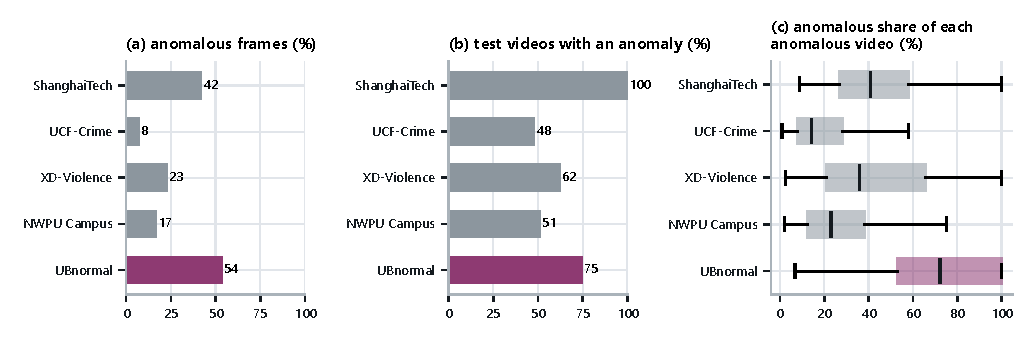
\includegraphics[width=\linewidth]{fig_p2_datasets}
\caption{The five test splits at a glance, computed from the frame labels at the
sampling used for scoring (UBnormal: every frame). (a) Share of anomalous frames. (b)
Share of test videos that contain any anomaly. (c) For videos that contain an anomaly,
the share of the video it covers (box: quartiles; whiskers: range).}\label{fig:datasets}
\end{figure}

\subsection{Evaluation metrics and uncertainty}
\label{sec:metrics}
Anomalies are rare in most benchmarks (Fig.~\ref{fig:datasets}a), so accuracy is
uninformative, and every measure used here is threshold-free. Let $\mathcal{A}$ and
$\mathcal{N}$ be the anomalous and normal frames being evaluated, with smoothed scores
$\tilde{s}_i$.

\emph{Frame-level AUROC} is the probability that an anomalous frame scores above a normal
one,
\begin{equation}
\mathrm{AUROC}=\frac{1}{|\mathcal{A}|\,|\mathcal{N}|}\sum_{i\in\mathcal{A}}\sum_{j\in\mathcal{N}}
\Big(\mathbf{1}[\tilde{s}_i>\tilde{s}_j]+\tfrac12\,\mathbf{1}[\tilde{s}_i=\tilde{s}_j]\Big),
\label{eq:auroc2}
\end{equation}
so $0.5$ is chance and $1$ a perfect ranking. The \emph{micro} AUROC pools the frames of
all videos into one ranking; it is the convention on every benchmark used here and the
figure reported unless stated otherwise. The \emph{macro} AUROC applies
Equation~\eqref{eq:auroc2} within each video $v$ and averages over the $V$ videos,
\begin{equation}
\mathrm{AUROC}_{\mathrm{macro}}=\frac{1}{V}\sum_{v=1}^{V}\mathrm{AUROC}\big(\mathcal{A}_v,\mathcal{N}_v\big),
\label{eq:macro}
\end{equation}
which a per-video shift of all scores cannot change. On UBnormal the macro figure
follows the authors' evaluation code, which pads every video with one normal and one
anomalous frame so that videos with a single class can be scored.

\emph{Average precision} is XD-Violence's official measure,
\begin{equation}
\mathrm{AP}=\int_0^1 \mathrm{P}(r)\,\mathrm{d}r,\qquad
\mathrm{P}(\tau)=\frac{|\{i\in\mathcal{A}:\tilde{s}_i\ge\tau\}|}{|\{i:\tilde{s}_i\ge\tau\}|},\quad
r(\tau)=\frac{|\{i\in\mathcal{A}:\tilde{s}_i\ge\tau\}|}{|\mathcal{A}|},
\label{eq:ap2}
\end{equation}
computed as the official code does, with each 16-frame snippet's score assigned to its
frames.

\emph{Scoring every frame on UBnormal.} UBnormal's protocol labels every frame, while the
detector scores every sixteenth. Each sampled frame's smoothed score is held for the
fifteen frames that follow it,
\begin{equation}
\hat{s}_{u} \;=\; \tilde{s}_{\lfloor u/16\rfloor}, \qquad u=0,1,\dots,U-1,
\label{eq:hold}
\end{equation}
where $u$ indexes all $U$ frames of the video and $\tilde{s}$ is indexed from zero, and
the last sampled score is held to the end. This choice was fixed before the test; the
AUROC over the sampled frames alone differs by at most $0.003$ for any condition
(Table~\ref{tbl:sealed}).

\emph{Uncertainty.} Frames within a video are strongly correlated, so uncertainty comes
from resampling whole videos. For two conditions $a$ and $b$ scored on the same $n$ test
videos, $B=1000$ resamples $\mathcal{V}^{(1)},\dots,\mathcal{V}^{(B)}$ of $n$ videos are
drawn with replacement (fixed seed), both conditions are scored on each, and
\begin{equation}
\Delta^{(k)} = M_a\big(\mathcal{V}^{(k)}\big)-M_b\big(\mathcal{V}^{(k)}\big),\qquad
\mathrm{CI}_{95} = \big[\,q_{0.025}(\Delta),\;q_{0.975}(\Delta)\,\big],
\label{eq:boot}
\end{equation}
with $q$ the empirical quantile. A difference is \emph{significant} when its interval
excludes zero. Pairing removes the variation that both conditions share, so a paired
interval is much narrower than the two separate intervals would suggest.

\subsection{The development round and its rule}
\label{sec:rule}
Development changed one thing at a time on the frozen encoder. Before each step, the
condition to be added, the reference it was compared with, the predictions and the
decision rule were committed to the repository; only then was the step scored. A
change $x$ was kept over the current best $b$ only if the paired differences
$\Delta_d = M_d(x)-M_d(b)$ over the four development benchmarks $d$ satisfied
\begin{equation}
\#\{d:\Delta_d>0\} > 2, \qquad
\#\{d:\mathrm{CI}_d \subset (0,\infty)\} \ge 2, \qquad
\#\{d:\mathrm{CI}_d \subset (-\infty,0)\} = 0 .
\label{eq:rule}
\end{equation}
A change must help on most benchmarks, clearly on at least two, and clearly hurt on
none. Each run first reproduced the stored scores of the current best to within
$10^{-5}$ before scoring anything new. Algorithm~\ref{alg:protocol} summarises the whole
procedure, from the first development step to the sealed result.

\begin{algorithm}[t]
\caption{Development under committed rules, then one sealed test}\label{alg:protocol}
\begin{algorithmic}[1]
\Require candidate changes $x_1, x_2, \dots$ in a fixed order; development set $\mathcal{D}_{\mathrm{dev}}$; keep rule (Eq.~\ref{eq:rule})
\State $b \gets$ plain PE-Core with the base prompts
\For{each candidate $x$}
  \State commit to Git: $x$, the reference $b$, the predictions and the rule \Comment{before any score of $x$ exists}
  \State \textbf{if} the stored scores of $b$ are not reproduced within $10^{-5}$ \textbf{then stop}
  \State score $x$ and $b$ on $\mathcal{D}_{\mathrm{dev}}$; paired bootstrap intervals $\mathrm{CI}_d$ (Eq.~\ref{eq:boot})
  \State \textbf{if} the rule passes \textbf{then} $b \gets x$ \Comment{kept}; report $x$ either way
\EndFor
\State freeze: record the hashes of the files that define $b$, the test protocol, the predictions and the permitted wording
\State commit the test code with its gates; only then obtain $\mathcal{D}_{\mathrm{test}}$
\State \textbf{if} any hash differs or the development scores are not reproduced \textbf{then stop}
\State score $b$ on $\mathcal{D}_{\mathrm{test}}$ once; report the result in the pre-registered wording
\end{algorithmic}
\end{algorithm}

\subsection{Freezing and the sealed test}
\label{sec:freeze}
When the round ended, the chosen configuration was frozen: the hashes of the seven
files that define it were recorded, together with the UBnormal protocol, the three
predictions, and a table stating exactly which sentence each possible outcome would
permit. The code for the sealed test, including a self-test on synthetic data and
gates that refuse to run if any frozen file has changed or the development scores are
not reproduced, was committed next. Only then was UBnormal downloaded. It was scored
once, and the script refuses a second run except for a recorded technical failure.
Figure~\ref{fig:timeline} shows the sequence with the commit of each step.

\begin{figure}[pos=htbp]
\centering
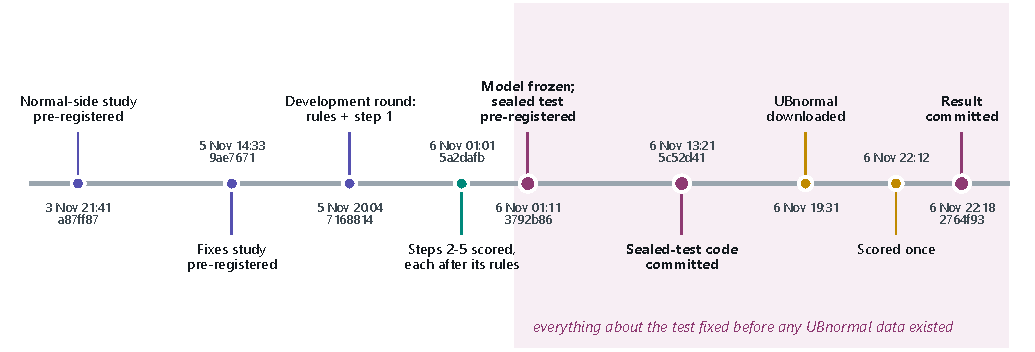
\includegraphics[width=\linewidth]{fig_p2_timeline}
\caption{The evidence chain, with the time and commit of each step (all times
6~November~2026 unless marked). Everything that determines the sealed result, from
the model's files to the words allowed for each outcome, was committed before the
first UBnormal file existed on any of our machines.}\label{fig:timeline}
\end{figure}

\subsection{Implementation}
All experiments ran on one NVIDIA A40 GPU under PyTorch 2.3.1. Both encoders are loaded
through \texttt{open\_clip} with their released weights and preprocessing:
PE-Core-L/14 at $336\times336$ pixels and CLIP ViT-L/14 trained on LAION-2B. Image
embeddings are computed once per benchmark and cached, separately from scores, because the
image encoder is the only expensive step and does not depend on the text; every text
condition in this paper is then scored from the same cached embeddings, which is also
what makes the reproduction gates exact. Each run writes a manifest with the code
commit, whether the working tree was clean, the hardware, the library versions, the
configuration and the frame and label counts of each benchmark. The bootstrap uses
1000 resamples with seed 20261104 throughout.

% =====================================================================
\section{Development Results}
\label{sec:dev}
% =====================================================================

\subsection{From the description-based system to the fixed prior}
Table~\ref{tbl:dev} and Fig.~\ref{fig:progression} follow the five configurations
that matter, on the same test videos. The first two rows are the first study's
detector, with and without a description generated by LLaVA for each camera or
video; the last row is the model of Section~\ref{sec:method}.

\begin{table}[width=\linewidth,cols=5,pos=htbp]
\caption{The development round on the same test videos: AUROC, and average precision
on XD-Violence. Rows after the second use no description and no captioning model.
The last row is the configuration that was frozen. These figures guided the design
and are exploratory.}\label{tbl:dev}
\begin{tabularx}{\linewidth}{@{}Z c c c c@{}}
\toprule
\textbf{Configuration} & \textbf{ShanghaiTech} & \textbf{UCF-Crime} & \textbf{XD-Violence} & \textbf{NWPU Campus} \\
\midrule
CLIP ViT-L/14, no text beyond the base prompts & 0.707 & 0.756 & 0.624 & 0.659 \\
CLIP ViT-L/14 + LLaVA description \citep{sarangi2026concept} & 0.751 & 0.824 & 0.417 & 0.667 \\
PE-Core, base prompts only & 0.666 & 0.847 & 0.494 & 0.617 \\
PE-Core + calm normal phrases (C) & 0.757 & 0.817 & 0.635 & 0.669 \\
\textbf{PE-Core + C + action bank (B)} & \textbf{0.783} & \textbf{0.856} & \textbf{0.722} & 0.639 \\
\bottomrule
\end{tabularx}
\end{table}

\begin{figure}[pos=htbp]
\centering
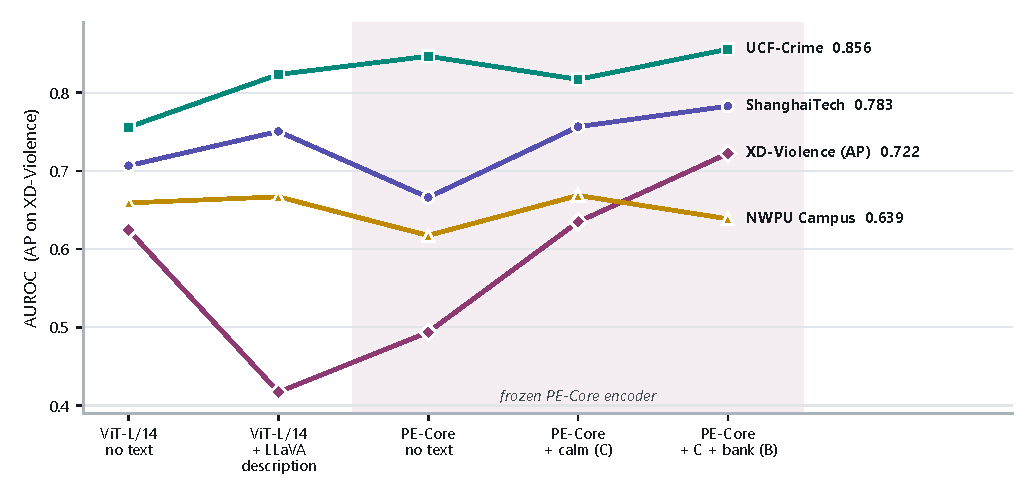
\includegraphics[width=\linewidth]{fig_p2_progression}
\caption{Table~\ref{tbl:dev} as a slope chart. Changing the encoder alone helps only
UCF-Crime; the calm phrases and the bank then recover and exceed the earlier system on
three of four benchmarks, most strongly on XD-Violence, where the description had
failed.}\label{fig:progression}
\end{figure}

\paragraph{The encoder alone is not the improvement.} Replacing CLIP ViT-L/14 by
PE-Core with the base prompts unchanged raises UCF-Crime by $+0.091\ci{+0.015}{+0.174}$
but lowers XD-Violence by $-0.131\ci{-0.181}{-0.079}$, and changes ShanghaiTech
($-0.041$) and NWPU Campus ($-0.042$) within noise. A stronger encoder does not by
itself make a better detector; what it offers is a text space in which the phrases
below can work.

\subsection{What each piece of text contributes}
\label{sec:dev-effects}
Table~\ref{tbl:effects} and Fig.~\ref{fig:forest} give every paired effect with its
interval.

\begin{table}[width=\linewidth,cols=6,pos=htbp]
\caption{Paired effects with 95\% video-level bootstrap intervals (AUROC; AP on
XD-Violence; micro AUROC on UBnormal). Bold: interval excludes zero. The UBnormal
column comes from the sealed run; a dash means that comparison was not part of
it.}\label{tbl:effects}
\scriptsize
\begin{tabularx}{\linewidth}{@{}Z c c c c c@{}}
\toprule
\textbf{Effect} & \textbf{ShanghaiTech} & \textbf{UCF-Crime} & \textbf{XD-Violence} & \textbf{NWPU Campus} & \textbf{UBnormal} \\
\midrule
PE-Core $-$ ViT-L/14, base prompts & $-0.041$ & $\mathbf{+0.091}$ & $\mathbf{-0.131}$ & $-0.042$ & --- \\
 & $[-0.085, +0.002]$ & $[+0.015, +0.174]$ & $[-0.181, -0.079]$ & $[-0.119, +0.029]$ & \\
\addlinespace
Calm phrases on PE-Core (C $-$ plain) & $\mathbf{+0.091}$ & $-0.030$ & $\mathbf{+0.141}$ & $\mathbf{+0.051}$ & $\mathbf{+0.036}$ \\
 & $[+0.044, +0.142]$ & $[-0.085, +0.024]$ & $[+0.106, +0.170]$ & $[+0.008, +0.099]$ & $[+0.006, +0.069]$ \\
\addlinespace
Second calm wording on PE-Core & $\mathbf{+0.057}$ & $-0.012$ & $\mathbf{+0.129}$ & $\mathbf{+0.052}$ & --- \\
 & $[+0.024, +0.094]$ & $[-0.057, +0.033]$ & $[+0.096, +0.157]$ & $[+0.014, +0.091]$ & \\
\addlinespace
Calm phrases on ViT-L/14 & $+0.017$ & $-0.021$ & $-0.011$ & $-0.006$ & --- \\
 & $[-0.005, +0.040]$ & $[-0.073, +0.028]$ & $[-0.036, +0.015]$ & $[-0.041, +0.030]$ & \\
\addlinespace
Bank on top of C (B $-$ C) & $+0.026$ & $\mathbf{+0.039}$ & $\mathbf{+0.088}$ & $-0.030$ & $\mathbf{+0.060}$ \\
 & $[-0.010, +0.062]$ & $[+0.006, +0.074]$ & $[+0.067, +0.109]$ & $[-0.066, +0.001]$ & $[+0.016, +0.102]$ \\
\addlinespace
Final $-$ description-based system & $+0.032$ & $+0.032$ & $\mathbf{+0.305}$ & $-0.028$ & --- \\
 & $[-0.006, +0.070]$ & $[-0.018, +0.087]$ & $[+0.255, +0.359]$ & $[-0.091, +0.031]$ & \\
\addlinespace
Final $-$ plain PE-Core & --- & --- & --- & --- & $\mathbf{+0.096}$ \\
 & & & & & $[+0.051, +0.142]$ \\
\addlinespace
Final $-$ plain ViT-L/14 & --- & --- & --- & --- & $\mathbf{+0.161}$ \\
 & & & & & $[+0.112, +0.215]$ \\
\bottomrule
\end{tabularx}
\end{table}

\begin{figure}[pos=htbp]
\centering
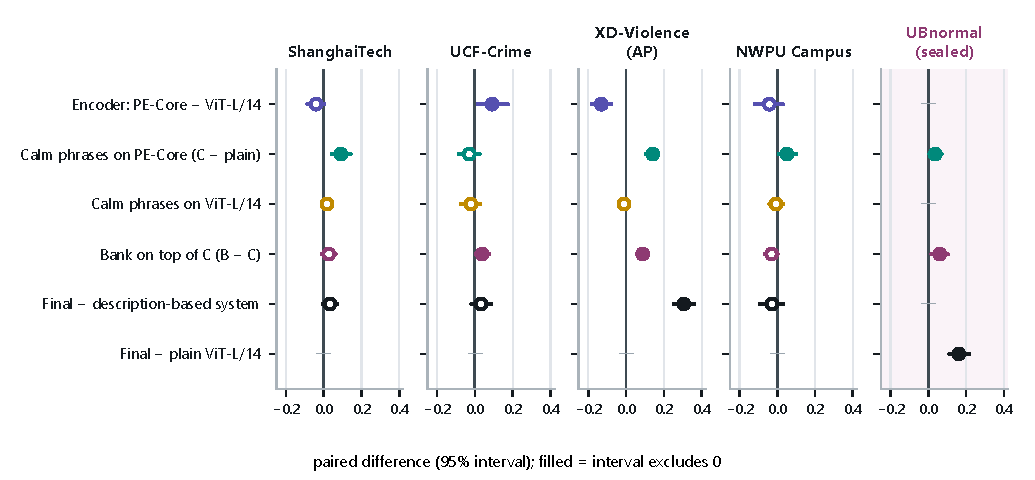
\includegraphics[width=\linewidth]{fig_p2_forest}
\caption{Table~\ref{tbl:effects} drawn: one panel per benchmark, one row per effect.
A filled circle means the 95\% interval excludes zero. The calm phrases help on
PE-Core and not on ViT-L/14; the bank adds most on XD-Violence; and the sealed
UBnormal panel (right) shows the same signs as development.}\label{fig:forest}
\end{figure}

\paragraph{Calm phrases.} On PE-Core the eight calm phrases raise ShanghaiTech,
XD-Violence and NWPU Campus significantly and leave UCF-Crime within noise, which
passes the rule of Equation~\eqref{eq:rule}. The second wording, which shares no
phrase with the first, passes it too, with the same three significant gains; the two
wordings differ significantly on ShanghaiTech and UCF-Crime, so the size of the
effect depends on the words, but its direction does not.

\paragraph{The effect depends on the encoder.} The same eight phrases do nothing
measurable on CLIP ViT-L/14: all four intervals contain zero. A text prior is
therefore not a property of the words alone but of the words in a particular
embedding space. We return to this in Section~\ref{sec:discussion}.

\paragraph{The action bank.} Replacing the three abstract abnormal phrases by the 48
concrete actions, on top of C, adds significantly on UCF-Crime and XD-Violence and
changes ShanghaiTech and NWPU Campus within noise, which passes the rule. Against the
first study's description-based system on the same videos, the final model is no
worse on any benchmark and better on XD-Violence by $+0.305$, the benchmark on which
the descriptions had failed.

\subsection{Re-ranking on two benchmarks}
\label{sec:dev-audit}
The first study introduced a measurement audit that splits a gain in pooled AUROC
into a \emph{level} part, which a per-video shift of the scores reproduces, and the
remainder, and that separately measures the change in AUROC within each video
\citep{sarangi2026concept}. There, $82$--$87\%$ of a description's gains were level.
The calm phrases behave differently. On ShanghaiTech their gain is re-ranking-dominated,
and AUROC within each video rises by $+0.166$; on NWPU Campus it is also
re-ranking-dominated (within-video $+0.070$). On XD-Violence, where many videos
contain no anomaly at all, the gain is mainly calibration, and on UCF-Crime, where the
calm phrases did not help ($-0.030$), the audit is mixed. On the two benchmarks where
re-ranking dominates, the calm phrases meet requirement R3 where the descriptions did
not: they change which frames within a video score high, not only how each video's
scores sit against the others.

\subsection{Curves on the development benchmarks}
Figure~\ref{fig:devroc} shows the full ROC and precision--recall curves of the final
model against the two plain encoders. The curves reproduce the areas of
Table~\ref{tbl:dev} to within $0.001$. On ShanghaiTech the final model lies above both
baselines at every false-positive rate; on XD-Violence its precision is higher at
almost every recall; on UCF-Crime its curve coincides with plain PE-Core's; on NWPU
Campus the three curves cross.

\begin{figure}[pos=htbp]
\centering
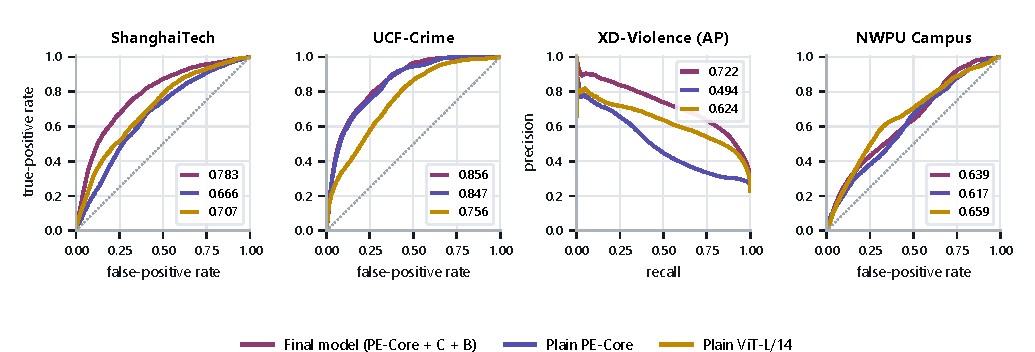
\includegraphics[width=\linewidth]{fig_p2_dev_roc}
\caption{ROC curves on ShanghaiTech, UCF-Crime and NWPU Campus and the
precision--recall curve on XD-Violence, for the final model and the two plain
encoders. Legends give the area of each curve (AUROC; AP on XD-Violence).}
\label{fig:devroc}
\end{figure}

\subsection{Score curves on single videos}
\label{sec:dev-qual}
Areas under curves summarise thousands of frames. Figure~\ref{fig:qual} shows what the
scores look like inside single test videos. To avoid choosing examples by eye, each video
was picked by a rule, stated in the caption, applied to the within-video AUROC.

\begin{figure}[pos=htbp]
\centering
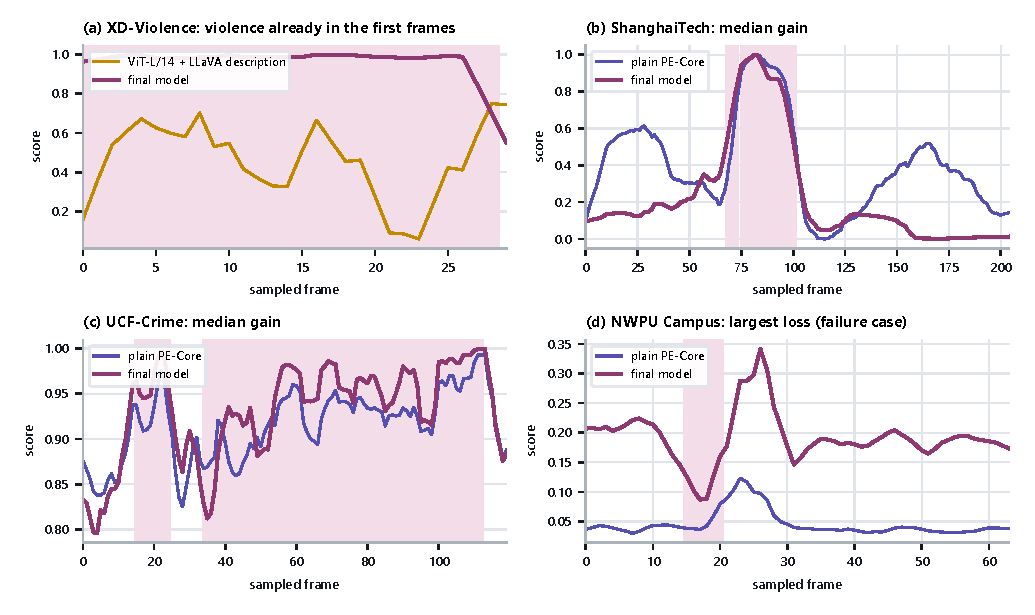
\includegraphics[width=\linewidth]{fig_p2_qualitative}
\caption{Smoothed scores inside four development test videos; shading marks the
labelled anomaly. (a) XD-Violence, against the first study's ViT-L/14 + LLaVA system:
of the videos violent within their first three sampled frames, the one with the largest
gain (a film excerpt). (b) ShanghaiTech and (c) UCF-Crime, against plain PE-Core: the
video with the median gain. (d) NWPU Campus, against plain PE-Core: the video with the
largest loss, a failure case.}\label{fig:qual}
\end{figure}

Panel (a) is the first study's failure in one video. The description, written from frames
that already show the fight, tells the detector the fight is normal, and its score stays
low and erratic throughout; the fixed prior scores the whole event high. Panel (b) shows
the typical gain on campus footage: both detectors find the event, but the final model
suppresses the two broad rises of plain PE-Core outside it, which is the within-video
re-ranking measured in Section~\ref{sec:dev-audit}. Panel (c) shows the typical UCF-Crime
video, where the two detectors largely agree. Panel (d) is the worst case on NWPU Campus:
the final model's score falls during the labelled event and peaks just after it, while
plain PE-Core barely moves. A fixed list has no way to know what
this scene's labels count as anomalous, the limitation discussed in
Section~\ref{sec:discussion}.

\subsection{What was tried and not kept}
\label{sec:dev-failed}
Table~\ref{tbl:round} lists every step of the round, in order. Three failures carry a
lesson. \emph{Scoring by anomaly type}, taking the highest of twelve type-wise scores
in the manner of NOVA \citep{yin2026nova}, raises XD-Violence to $0.769$ but lowers
ShanghaiTech by $-0.082\ci{-0.138}{-0.025}$: text sharpened for crime footage costs
accuracy on campus footage. \emph{Choosing the bank's types from each camera's scene},
matched without labels from five calm frames, recognises scenes sensibly (eleven of
the twelve ShanghaiTech cameras choose ``a pedestrian walkway on a campus''), and a
deliberately wrong scene is significantly worse than the whole bank on all four
benchmarks; but the right scene adds nothing over the whole bank. \emph{Novelty
against the camera's own past}, comparing each frame with a memory of the camera's
earlier frames, costs $-0.033$ on ShanghaiTech and $-0.117$ on XD-Violence. Before the
round, a pre-registered study had also tested NOVA's \emph{visual normal anchor}, a
mean image vector from five calm frames of each video mixed into the normal side
\citep{yin2026nova}. On PE-Core it gained $+0.013\ci{+0.000}{+0.026}$ on UCF-Crime but
lost $-0.037\ci{-0.058}{-0.016}$ on XD-Violence, and was not kept: like the scene
descriptions of the first study, a reference taken from each video's own frames is only
as normal as those frames.

\begin{table}[width=\linewidth,cols=3,pos=htbp]
\caption{Every step of the development round, in order, each judged against the
current best by the rule of Equation~\eqref{eq:rule}.}\label{tbl:round}
\small
\begin{tabularx}{\linewidth}{@{}l Z Z@{}}
\toprule
\textbf{Step} & \textbf{Change} & \textbf{Outcome} \\
\midrule
1 & Second wording of the calm phrases & passes: the calm phrases are kept \\
1 & ``Normal scene:'' / ``Anomalous scene:'' prefixes on top of C & fails: NWPU Campus $-0.014\ci{-0.026}{-0.003}$ \\
2 & PE-Core and ViT-L/14 margins averaged & fails: significant gain on XD-Violence only \\
3 & Frozen bank of concrete actions (B) & \textbf{passes: kept} \\
3 & Bank scored by anomaly type & fails: ShanghaiTech $-0.082$ \\
3 & Different templates for each side \citep{lee2025flashback} & fails: NWPU Campus $-0.026\ci{-0.049}{-0.007}$ \\
4 & Bank types chosen from each camera's scene & fails: all differences within noise \\
5 & Novelty against the camera's own past frames & fails: ShanghaiTech $-0.033$, XD-Violence $-0.117$ \\
6 & Per-video baseline subtraction & not run; the reason was recorded before the round closed \\
\bottomrule
\end{tabularx}
\end{table}

% =====================================================================
\section{The Sealed Test on UBnormal}
\label{sec:sealed}
% =====================================================================

\subsection{Why UBnormal, and what was fixed}
UBnormal \citep{acsintoae2022ubnormal} is built from 29 rendered scenes, and its test
anomalies are of types that its training anomalies are not. It played no part in any
choice: it was named as the held-out benchmark before development began, and it was
downloaded only after the freeze. Its test split contains twelve anomaly types, none of which appears in its training
split: running, having a seizure, laying down, shuffling, walking drunk, a person hit
by a car, a car crash, jumping, fire, smoke, jaywalking and driving outside the lane
\citep{acsintoae2022ubnormal}. The bank names some of these, such as a car crash,
fire, smoke, running and a person lying on the ground, and does not name others,
such as a seizure, shuffling, walking drunk, jaywalking or driving outside the lane. Three predictions were registered with the freeze
(Table~\ref{tbl:pred}), as was a table of permitted wording: the sentence the result
would allow for detection, for transfer of the text prior, and for the comparison with
the original encoder.

\subsection{Result}
Before scoring, the gates passed: the seven frozen files matched their hashes, the
frozen model reproduced its development scores exactly on all four benchmarks, all 211
test videos and their annotation files were present, and the sampled labels agreed
with the frame-level labels. The run covered all 92{,}640 test frames, of which 49{,}850
are anomalous. Table~\ref{tbl:sealed} gives the result.

\begin{table}[width=\linewidth,cols=5,pos=htbp]
\caption{The sealed test on the UBnormal test split, scored once. Micro AUROC over
all 92{,}640 frames is the pre-registered primary measure; intervals are 95\%
video-level bootstrap intervals over the 211 videos.}\label{tbl:sealed}
\begin{tabularx}{\linewidth}{@{}Z c c c c@{}}
\toprule
\textbf{Condition} & \textbf{Micro AUROC} & \textbf{95\% interval} & \textbf{Macro AUROC} & \textbf{Sampled frames} \\
\midrule
\textbf{Final model (PE-Core + C + B)} & \textbf{0.747} & \textbf{[0.704, 0.789]} & \textbf{0.906} & \textbf{0.749} \\
PE-Core + calm phrases (C) & 0.687 & [0.634, 0.741] & 0.896 & 0.690 \\
Plain PE-Core & 0.651 & [0.599, 0.708] & 0.858 & 0.654 \\
Plain CLIP ViT-L/14 & 0.586 & [0.522, 0.644] & 0.813 & 0.588 \\
\bottomrule
\end{tabularx}
\end{table}

\begin{table}[width=\linewidth,cols=3,pos=htbp]
\caption{Predictions registered with the freeze, and their outcomes.}\label{tbl:pred}
\small
\begin{tabularx}{\linewidth}{@{}Z l l@{}}
\toprule
\textbf{Prediction} & \textbf{Measured} & \textbf{Outcome} \\
\midrule
U1: the final model's 95\% interval lies above 0.5 & $[0.704, 0.789]$ & holds \\
U2: final $-$ plain PE-Core is above 0 & $+0.096$ & holds \\
U3: the final model's micro AUROC lies between 0.60 and 0.75 & $0.747$ & holds, narrowly \\
\bottomrule
\end{tabularx}
\end{table}

The text prior carried over. The calm phrases add $+0.036\ci{+0.006}{+0.069}$ to plain
PE-Core, the bank adds a further $+0.060\ci{+0.016}{+0.102}$, and together they add
$+0.096\ci{+0.051}{+0.142}$; the final model exceeds plain ViT-L/14 by
$+0.161\ci{+0.112}{+0.215}$. Every effect has the sign it had in development
(Fig.~\ref{fig:forest}, right panel), and none of the three predictions failed.

In the wording fixed before the test, the result permits three statements: the model
\emph{detects anomalies on an unseen dataset, without training}; \emph{the calm phrases
and bank carried over to unseen data}; and, against plain ViT-L/14, it is \emph{no
worse}. The last is deliberately weak. The rule that would permit ``better'' requires
significant gains on two benchmarks, and a single benchmark cannot satisfy it; we apply
it as written, although the interval of the difference lies well above zero.

\subsection{Where the score comes from}
\label{sec:sealed-posthoc}
The analyses in this subsection were not pre-registered. They were run after the
sealed result was recorded, on per-frame scores exported by a script that first
reproduced all four sealed micro AUROCs exactly, and they describe the result rather
than test anything.

\begin{figure}[pos=htbp]
\centering
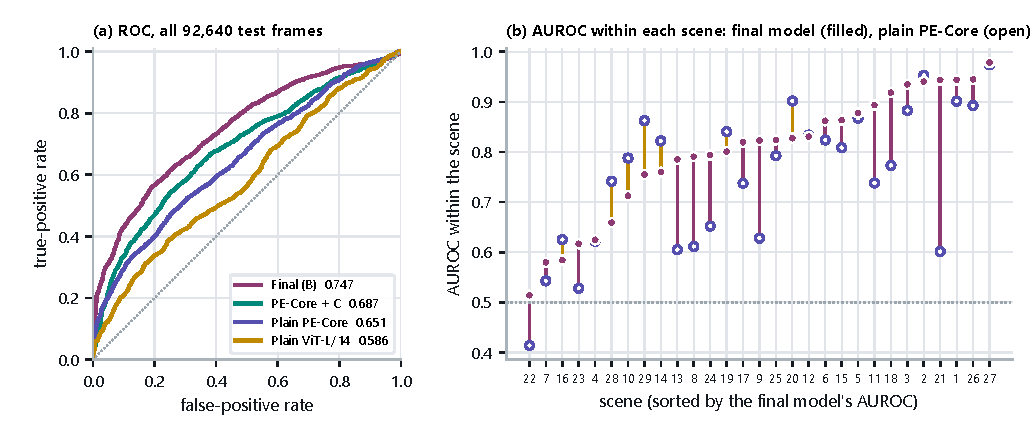
\includegraphics[width=\linewidth]{fig_p2_ubnormal}
\caption{The sealed test in detail. (a) ROC curves of the four conditions over all
test frames; legends give the sealed micro AUROC. (b) AUROC within each scene that
contains both normal and anomalous frames, for the final model (filled) and plain
PE-Core (open), scenes sorted by the final model's score. Post hoc.}
\label{fig:ubnormal}
\end{figure}

Figure~\ref{fig:ubnormal}(a) shows that the final model's advantage holds across the
whole ROC curve rather than at one operating point. Figure~\ref{fig:ubnormal}(b)
breaks the result down by scene: in 20 of the 29 scenes that contain both normal and anomalous frames the final model ranks frames better than plain PE-Core, the median within-scene AUROC rises from $0.788$ to $0.823$, and the final model stays above chance in every scene (lowest $0.514$), where plain PE-Core falls below it in one. The gain is spread across scenes rather than carried by a few, as a text prior that does not depend on the scene should produce.

Figure~\ref{fig:types} asks which of the bank's twelve types carry the signal on data
whose anomalies the bank names only in part. Each type's four phrases, set against the
normal side, form a one-type detector. All 12 types rank anomalous frames above normal ones better than chance. The strongest is \emph{falling} ($0.766$), whose phrases describe people collapsing or lying on the ground, which is close to the test split's ``having a seizure'' and ``laying down''; it is followed by \emph{abuse} ($0.723$) and \emph{riot or arrest} ($0.711$). The weakest is \emph{vehicle among pedestrians} ($0.542$), even though the test split contains jaywalking and driving outside the lane: phrases about cyclists and cars among pedestrians may not capture a pedestrian crossing a road. The whole bank ($0.744$ under the same unsmoothed conditions) is close to its best type and well above its average one, so its strength on this data comes from breadth rather than from one well-chosen phrase.

\begin{figure}[pos=htbp]
\centering
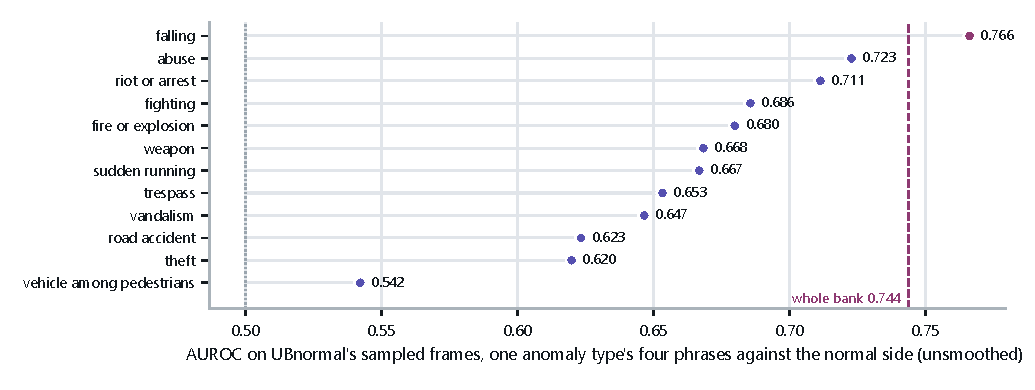
\includegraphics[width=\linewidth]{fig_p2_ubnormal_types}
\caption{Each anomaly type of the bank used alone against the normal side, on
UBnormal's sampled frames without smoothing; the dashed line is the whole bank under
the same conditions. Post hoc and descriptive.}\label{fig:types}
\end{figure}

\subsection{Against published UBnormal results}
Table~\ref{tbl:sota-ub} lists the published figures we could verify in their source
papers; all are micro frame-level AUROC on the test split, the same measure as ours.
Every method listed uses UBnormal's own training data, and none is training-free.

\begin{table}[width=\linewidth,cols=4,pos=htbp]
\caption{Published results on the UBnormal test split (\%). $^{a}$As reported with the
benchmark \citep{acsintoae2022ubnormal}, Table~2. $^{b}$As tabulated by
\citet{yang2024anomalyruler}, Table~3, whose UBnormal column gives the micro figure
(its entry for Georgescu et al.\ equals that method's micro AUROC in
\citet{acsintoae2022ubnormal}). $^{c}$\citet{wu2024ovvad}, Table~3. A dash means not
reported.}\label{tbl:sota-ub}
\small
\begin{tabularx}{\linewidth}{@{}Z l c c@{}}
\toprule
\textbf{Method} & \textbf{Uses from UBnormal} & \textbf{Micro} & \textbf{Macro} \\
\midrule
Georgescu et al.$^{a}$ & normal training videos & 59.3 & 84.9 \\
Georgescu et al. + UBnormal anomalies$^{a}$ & training videos and anomalies & 61.3 & 85.6 \\
Bertasius et al. (1/32 sample rate, fine-tuned)$^{a}$ & supervised fine-tuning & 68.5 & 80.3 \\
FPDM$^{b}$ & normal training videos & 62.7 & --- \\
OVVAD$^{c}$ & training videos & 62.94 & --- \\
STG-NF$^{b}$ & normal training videos & 71.8 & --- \\
AnomalyRuler$^{b}$ & a few normal frames, and GPT-4 & 71.9 & --- \\
\midrule
\textbf{DA-ZVAD v2, final (ours)} & \textbf{nothing} & \textbf{74.7} & \textbf{90.6} \\
\bottomrule
\end{tabularx}
\end{table}

The final model's $74.7$ is above every published micro figure in the table, and its
macro $90.6$ is above every macro figure. Two of these margins are not established:
STG-NF's $71.8$ and AnomalyRuler's $71.9$ both lie inside our 95\% interval of
$[70.4, 78.9]$. We therefore say ``above'' and not ``better''. The figures are also not
equally earned: every published method has seen UBnormal's training data, and ours has
seen nothing of UBnormal at all.

% =====================================================================
\section{Ablation Study}
\label{sec:ablation}
% =====================================================================

The development round (Section~\ref{sec:dev}) added one component at a time and kept it
only if the rule passed. This section takes the finished model apart: each ingredient is
removed in turn, and each design choice is varied with the others held fixed. The
component ablation uses the development benchmarks and the sealed run; the design
ablations are computed after the sealed test, on UBnormal's per-frame features, by a
script that first reproduced all four sealed micro AUROCs exactly. They are post hoc,
describe the frozen model rather than test it, and were not used to change it.

\subsection{Removing each ingredient}
Table~\ref{tbl:ablation} removes the bank, the calm phrases, or both, and swaps the
encoder. Every ingredient is needed on the sealed test. Without the bank the model loses
$-0.060\ci{-0.102}{-0.016}$; without the calm phrases (the 48 actions against the three
general normal phrases) it loses $-0.090\ci{-0.127}{-0.052}$; without both it falls to
plain PE-Core, $-0.096\ci{-0.142}{-0.051}$. The order of importance matches development
on XD-Violence, where the calm phrases added $+0.141$ and the bank $+0.088$. The encoder
swap shows the other half of the result: the same eight calm phrases on CLIP ViT-L/14
change no development benchmark significantly, so neither the text nor the encoder
alone is the improvement; their combination is.

\begin{table}[width=\linewidth,cols=6,pos=htbp]
\caption{Component ablation: AUROC (AP on XD-Violence; micro AUROC on UBnormal). C:
eight calm normal phrases; B: the 48-action bank. $^{\dagger}$Computed after the sealed
test from the same features (post hoc); the other UBnormal entries are pre-registered
conditions of the sealed run. A dash means not run: development added B only on top of
C, and the sealed run did not include ViT-L/14 with C.}\label{tbl:ablation}
\small
\begin{tabularx}{\linewidth}{@{}Z c c c c c@{}}
\toprule
\textbf{Configuration} & \textbf{ShanghaiTech} & \textbf{UCF-Crime} & \textbf{XD-Violence} & \textbf{NWPU Campus} & \textbf{UBnormal} \\
\midrule
\textbf{Final: PE-Core + C + B} & \textbf{0.783} & \textbf{0.856} & \textbf{0.722} & 0.639 & \textbf{0.747} \\
$-$ bank (PE-Core + C) & 0.757 & 0.817 & 0.635 & \textbf{0.669} & 0.687 \\
$-$ calm phrases (PE-Core + B) & --- & --- & --- & --- & 0.657$^{\dagger}$ \\
$-$ both (plain PE-Core) & 0.666 & 0.847 & 0.494 & 0.617 & 0.651 \\
\midrule
CLIP ViT-L/14 + C & 0.724 & 0.735 & 0.614 & 0.653 & --- \\
CLIP ViT-L/14, base prompts & 0.707 & 0.756 & 0.624 & 0.659 & 0.586 \\
\bottomrule
\end{tabularx}
\end{table}

\subsection{Design choices}
Table~\ref{tbl:ablation-design} and Fig.~\ref{fig:ablation} vary one choice at a time on
UBnormal; differences are against the frozen model's $0.7475$, with paired intervals for
the phrase-set variants.

\begin{table}[width=\linewidth,cols=3,pos=htbp]
\caption{Design ablations on the UBnormal test split, micro AUROC over all frames. Post
hoc: computed after the sealed result and not used to change the model. Differences are
against the frozen model ($0.7475$); 95\% paired video-level intervals are given for the
phrase-set variants.}\label{tbl:ablation-design}
\small
\begin{tabularx}{\linewidth}{@{}Z c l@{}}
\toprule
\textbf{Variant (all else as frozen)} & \textbf{AUROC} & \textbf{Difference} \\
\midrule
\multicolumn{3}{@{}l}{\emph{Normal side (frozen: 3 general + 4 quiet places + 4 calm people)}} \\
8 calm phrases, without the 3 general & 0.756 & $+0.008\ci{-0.004}{+0.022}$ \\
3 general + 4 quiet places only & 0.708 & $\mathbf{-0.039}\ci{-0.055}{-0.025}$ \\
3 general + 4 calm people only & 0.749 & $+0.002\ci{-0.014}{+0.019}$ \\
\addlinespace
\multicolumn{3}{@{}l}{\emph{Abnormal side (frozen: 12 types $\times$ 4 actions)}} \\
Bank + the 3 general abnormal phrases & 0.748 & $+0.001\ci{-0.003}{+0.004}$ \\
First 1 / 2 / 3 phrases of each type & 0.715 / 0.731 / 0.744 & $-0.032$ / $-0.016$ / $-0.004$ \\
One type left out: worst (falling) / best (theft) & 0.731 / 0.752 & $-0.017$ / $+0.004$ \\
\addlinespace
\multicolumn{3}{@{}l}{\emph{Scoring (frozen: mean of phrase vectors, $\lambda=100$, $w=5$)}} \\
Log-mean-exp of phrase similarities / maximum similarity & 0.713 / 0.698 & $-0.035$ / $-0.050$ \\
$\lambda = 1$ / $10$ / $30$ / $300$ & 0.751 / 0.751 / 0.751 / 0.742 & $+0.003$ / $+0.003$ / $+0.003$ / $-0.006$ \\
$w = 1$ / $3$ / $9$ / $15$ / $31$ & 0.740 / 0.750 / 0.742 / 0.733 / 0.713 & $-0.008$ / $+0.002$ / $-0.005$ / $-0.015$ / $-0.034$ \\
\bottomrule
\end{tabularx}
\end{table}

\begin{figure}[pos=htbp]
\centering
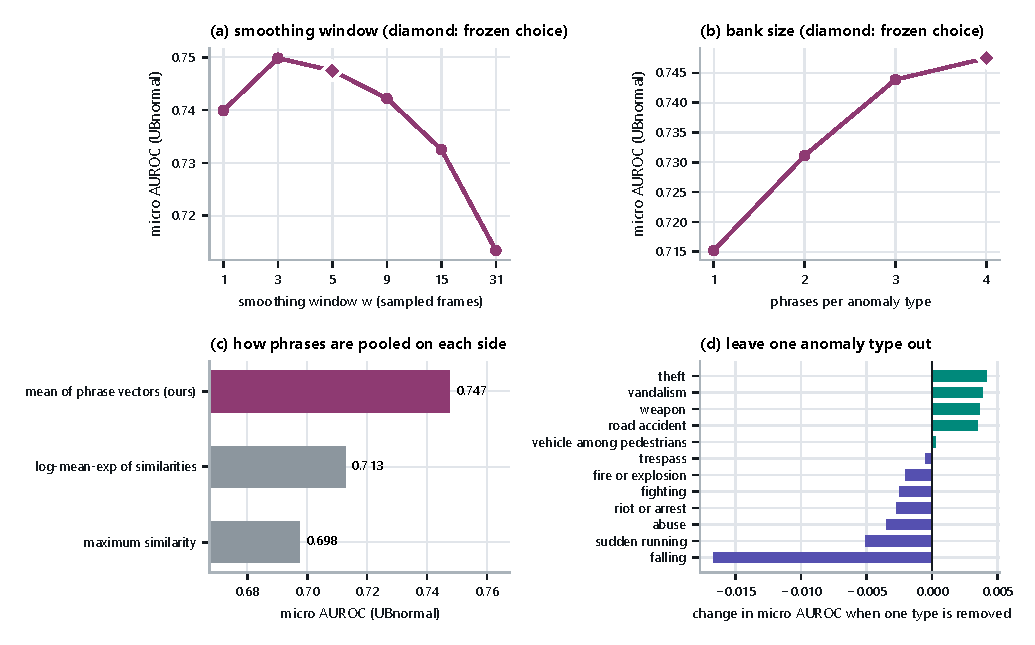
\includegraphics[width=\linewidth]{fig_p2_ablation}
\caption{Design ablations on UBnormal (post hoc). (a) Smoothing window. (b) Number of
phrases per anomaly type, keeping the first $k$ of each type. (c) How phrases are pooled
on each side. (d) Change in micro AUROC when one anomaly type's four phrases are removed.
Diamonds and purple bars mark the frozen choices.}\label{fig:ablation}
\end{figure}

\paragraph{Which calm phrases matter.} On UBnormal the four calm-people phrases carry the
normal side: keeping only the quiet places costs $-0.039$, significantly, while keeping
only the people costs nothing. The three general phrases from the first study could be
dropped (+0.008, within noise).

\paragraph{The bank works by breadth.} Every extra phrase per type helps, from $0.715$
with one to $0.747$ with four, and no single type carries the result: removing any one
changes the score by at most $0.017$. The largest loss comes from removing
\emph{falling}, the type closest to UBnormal's ``having a seizure'' and ``laying down''.
Removing four types (theft, vandalism, weapon, road accident) raises the score slightly,
by $0.004$ at most.

\paragraph{Pooling into one prototype is the right rule.} Comparing each frame with every
phrase and pooling the similarities, by the maximum or by a soft maximum, is worse by
$0.035$ to $0.050$. This repeats the first study's finding that per-prompt maximum
pooling lost to mean-pooled prototypes \citep{sarangi2026concept}: an average of many
phrases is a steadier reference than the single phrase a frame happens to match best.

\paragraph{Smoothing and temperature.} A window of three to five sampled frames is best,
and longer windows blur short events away ($-0.034$ at $w=31$). The temperature matters
little: the sigmoid is monotone, so $\lambda$ changes the ranking of frames only through
the smoothing that follows it.

\paragraph{What the ablation does not license.} Three variants score marginally above the
frozen model: no general phrases, $w=3$, and $\lambda\le30$. All differences are at most
$0.008$, the one tested is within noise, and all were found on the test set after the
fact. Choosing any of them now would be selection on the test data, which the sealed
protocol exists to prevent; a further change would need a new sealed test.

% =====================================================================
\section{Comparison Across Benchmarks}
\label{sec:compare}
% =====================================================================

Table~\ref{tbl:sota-final} and Fig.~\ref{fig:compare} place the final model among
published results on all five benchmarks. Every external figure was read from its
source paper and recorded with its location before being used.

\begin{table}[width=\linewidth,cols=6,pos=htbp]
\caption{The final model against published results (\%): AUROC, AP on XD-Violence,
micro AUROC on UBnormal. A dash means not reported. $^{\ast}$As tabulated by
\citet{yin2026nova}, Table~1. $^{\#}$As tabulated by \citet{lee2025flashback},
Table~1; VERA learns its questions on training data. $^{\P}$Uses a few normal target
frames and GPT-4. NWPU Campus figures as tabulated by \citet{cao2023nwpu}, Table~4,
computed over every frame where ours uses every sixteenth. Our development figures are
exploratory; our UBnormal figure is the sealed result.}\label{tbl:sota-final}
\scriptsize
\begin{tabularx}{\linewidth}{@{}Z c c c c c@{}}
\toprule
\textbf{Method} & \textbf{UCF-Crime} & \textbf{XD-Violence} & \textbf{ShanghaiTech} & \textbf{NWPU Campus} & \textbf{UBnormal} \\
\midrule
\multicolumn{6}{@{}l}{\emph{Training-free}} \\
NOVA \citep{yin2026nova} & 89.86 & 84.82 & --- & --- & --- \\
ASK-Hint \citep{zou2026askhint} & 89.83 & --- & --- & --- & --- \\
Flashback-PE \citep{lee2025flashback} & 87.29 & 75.13 & --- & --- & --- \\
\textbf{DA-ZVAD v2, final (ours)} & \textbf{85.6} & \textbf{72.2} & \textbf{78.3} & \textbf{63.9} & \textbf{74.7} \\
Frozen VLM, yes/no probability \citep{song2026vlmanswer} & 85.32 & 68.98 & --- & --- & --- \\
PANDA$^{\ast}$ & 84.89 & 70.16 & --- & --- & --- \\
VADTree$^{\ast}$ & 84.74 & 68.85 & --- & --- & --- \\
EventVAD$^{\ast}$ & 82.03 & 64.04 & --- & --- & --- \\
AnyAnomaly \citep{anyanomaly2025} & 80.7 & --- & 79.7 & --- & --- \\
LAVAD \citep{zanella2024lavad} & 80.3 & 62.01 & --- & --- & --- \\
\midrule
\multicolumn{6}{@{}l}{\emph{Using data from the target benchmark}} \\
VERA$^{\#}$ \citep{ye2025vera} & --- & 70.54 & --- & --- & --- \\
AnomalyRuler$^{\P}$ \citep{yang2024anomalyruler} & --- & --- & 85.2 & --- & 71.9 \\
MULDE \citep{micorek2024mulde} & 78.5 & --- & 81.3 & --- & --- \\
FPDM \citep{yan2023fpdm} & 74.7 & --- & 78.6 & --- & 62.7 \\
MPN \citep{lv2021mpn} & --- & --- & 73.8 & 64.4 & --- \\
Cao et al., scene-conditioned \citep{cao2023nwpu} & --- & --- & --- & 68.2 & --- \\
Cao et al., unconditioned \citep{cao2023nwpu} & --- & --- & --- & 65.8 & --- \\
AMMC-Net & --- & --- & --- & 64.5 & --- \\
HF2-VAD & --- & --- & --- & 63.7 & --- \\
MNAD & --- & --- & --- & 62.5 & --- \\
MemAE & --- & --- & --- & 61.9 & --- \\
STG-NF & --- & --- & --- & --- & 71.8 \\
OVVAD \citep{wu2024ovvad} & --- & --- & --- & --- & 62.94 \\
\bottomrule
\end{tabularx}
\end{table}

\begin{figure}[pos=htbp]
\centering
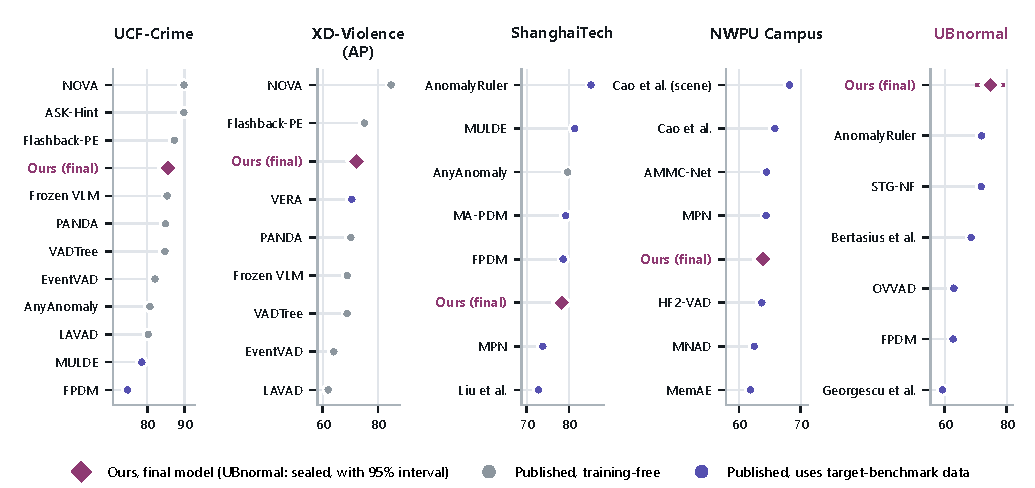
\includegraphics[width=\linewidth]{fig_p2_comparison}
\caption{Table~\ref{tbl:sota-final} as dot plots, one panel per benchmark, sorted by
score. Diamonds: the final model, with its 95\% interval on UBnormal. Grey: published
training-free methods. Blue: published methods that use data from the target
benchmark.}\label{fig:compare}
\end{figure}

Among training-free methods the final model is behind NOVA, ASK-Hint and Flashback-PE
on UCF-Crime, and behind NOVA and Flashback-PE on XD-Violence, and ahead of the rest. On
ShanghaiTech it lies among the one-class methods that train on that benchmark, and on
NWPU Campus inside the range of the trained methods reported with it. Three cautions
apply. Our intervals on the development benchmarks span several points, so gaps of one
or two points there are not differences. The development figures are exploratory, for
the reasons given in Section~\ref{sec:threats}. And the strongest methods are informed
differently: NOVA writes twenty normal and twenty anomalous phrases for each anomaly
class with guidance for each dataset \citep{yin2026nova}, Flashback retrieves from a
memory of a million generated captions using a video encoder \citep{lee2025flashback},
and ASK-Hint queries a large video-language model \citep{zou2026askhint}. We are not aware that any of them has been evaluated on a benchmark held out from
its own design, which is the setting in which our UBnormal figure was obtained.

% =====================================================================
\section{Discussion}
\label{sec:discussion}
% =====================================================================

\paragraph{Why might calm phrases help?} NOVA's account is that normal prompts
containing ambiguous verbs blur the boundary with anomalies \citep{yin2026nova}. Our
results add to it. Phrases such as ``a normal scene'' sit close to everything, so the
normal prototype barely separates quiet frames from busy ones; phrases about empty
places and still, unhurried people give it a specific direction, toward low motion and
few people, and anomalies in surveillance footage are mostly the opposite. That they help on PE-Core and not on ViT-L/14 suggests
that PE-Core's text space represents such states of a scene, as opposed to its
objects, more distinctly. We offer this as a hypothesis; the experiments here show the
dependence on the encoder but not its cause.

\paragraph{Why did NWPU Campus not improve?} The calm phrases raise NWPU Campus
significantly, but the bank then lowers it by $-0.030$, within noise, so the final
model ends below the first study's detector there. NWPU Campus contains anomalies that
are anomalous only in particular scenes, such as cycling on a footpath or a lorry in a
pedestrian area \citep{cao2023nwpu}, and a fixed list cannot know which scene forbids
what. This is the cost of requirement R1, and the first study's scene descriptions,
which did not help there either, did not pay it back.

\paragraph{What changed from the first study.} The first study's text told the
detector which scene it was looking at and mostly moved whole videos up or down. The
fixed prior tells it what ordinary and alarming footage look like in general, and on
two of the four benchmarks it mainly reorders frames within a video. It also removes the dependence on a camera's
opening frames, which was the cause of the XD-Violence failure, and the model that
results is simpler: no captioning model, no per-camera step, and one encoder pass per
sampled frame.

\subsection{Threats to validity}
\label{sec:threats}
\begin{itemize}
  \item \emph{Development reuse.} The four development benchmarks were used to choose
        the design, many conditions were scored on them, and their intervals are not
        corrected for multiple comparisons. Their figures are exploratory; only the
        UBnormal figure is a test.
  \item \emph{An informed bank.} The bank was written by a large language model that
        knew the anomaly types of the development benchmarks. The UBnormal paper, which
        lists its test anomaly types, had also been read (3~November~2026) before the
        bank was written (5~November~2026), in order to plan the sealed test. The bank
        was not written from that list, and no UBnormal video or label was seen before
        scoring, but the overlap between the bank and the list (a car crash, fire,
        smoke, running, a person on the ground) may owe something to it, or to general
        knowledge of what surveillance anomalies look like; we cannot separate the two.
  \item \emph{One synthetic test.} UBnormal is computer-generated, and a single
        benchmark is a single test. A good result supports the model; it does not show
        that it will hold on real footage from new sites.
  \item \emph{Held scores.} UBnormal is scored on every frame by holding each sampled
        frame's score for fifteen frames, as fixed before the test; the AUROC over the
        sampled frames alone ($0.749$) is almost identical.
  \item \emph{Narrow prediction.} U3 held by $0.003$; had the model scored slightly
        higher, that prediction would have failed while the result improved, which
        shows the prediction's range, set before any UBnormal data existed, was
        conservative rather than tuned.
\end{itemize}

\subsection{Limitations and future work}
The model scores whole frames, so anomalies too small or too brief to change a frame's
embedding are invisible to it; patch-level scoring is the obvious extension. Its text
cannot express scene-dependent rules, which is why NWPU Campus did not improve; a
second held-out benchmark with such rules, and real rather than rendered footage, are
the tests that remain. The calm phrases' dependence on the encoder should be examined
across more encoders, and the bank should be rewritten by a model that has not seen
any of the benchmarks, to measure how much of its success is general.

% =====================================================================
\section{Conclusion}
\label{sec:conclusion}
% =====================================================================

One fixed set of 59 phrases, written once and used unchanged on every camera, carries a
frozen detector as well as text written for each camera did on three of four
development benchmarks, and far better on the one where per-camera text failed. Its
calm normal phrases work only in the right embedding space, and on two benchmarks they
help mainly by reordering frames within a video rather than by calibrating cameras. Developed under committed
rules and frozen before a fifth benchmark was obtained, the model reached $0.747$ AUROC
on UBnormal, with the text prior adding $+0.096$ over the same encoder alone, and every
pre-registered prediction held. A training-free detector need not be told where it is;
it can be told, once, what calm footage looks like and what goes wrong.

\section*{Declaration of competing interest}
The authors declare that they have no known competing financial interests or personal
relationships that could have appeared to influence the work reported in this paper.

\section*{Data and code availability}
All benchmarks are public and are used under their authors' terms; UBnormal is used
under CC BY-NC-ND 4.0, and no frame, video or label of it is redistributed. The code,
the pre-registration documents with their dated addenda, the frozen file hashes, run
manifests and per-condition results will be made available on publication.

\section*{Declaration of generative AI and AI-assisted technologies in the writing process}
% CONFIRM THE WORDING WITH THE SUPERVISORS BEFORE SUBMISSION.
During the preparation of this work the authors used Claude (Anthropic) to assist with
code, analysis and the drafting of text. The abnormal phrase bank was generated by a
large language model, as described in Section~\ref{sec:method}. After using these
tools, the authors reviewed and edited the content as needed and take full
responsibility for the content of the publication.

\section*{Acknowledgements}
The authors thank the Department of Computer Science and Engineering, National
Institute of Technology Calicut, for access to its GPU server.

\printcredits

\bibliographystyle{model1-num-names}
\bibliography{references}

\end{document}
